\section{pictureSlides}

\begin{frame}
    \begin{figure}[htp]
        \centering
        \includegraphics[width=.8\textwidth, keepaspectratio]{%
            % image has to be relative to the actual f4_beamer.tex because
            % this file is being included there. Hence, if the image is relative
            % to this current directory it will not work.
            pictureSlides/test-image.jpg}
        \caption{%
            https://www.pexels.com/de-de/foto/natur-dunkel-wald-baume-6992/
        }
    \end{figure}
\end{frame}

\begin{frame}
    \begin{figure}[!tbp]
        \centering
        % https://www.namsu.de/Extra/befehle/Minipage.html
        \begin{minipage}{0.5\textwidth}
            \includegraphics[width=\textwidth]{pictureSlides/test-image.jpg}
            \caption{picture number 1}
        \end{minipage}
        \hfill
        \begin{minipage}{0.4\textwidth}
            \includegraphics[width=\textwidth]{pictureSlides/test-image.jpg}
            \caption{picture number 2}
        \end{minipage}
        \caption{this is very interesting}
    \end{figure}
\end{frame}

\begin{frame}
    \begin{figure}[!tbp]
        \centering
        \begin{minipage}{0.4\textwidth}
            \includegraphics[width=\textwidth]{pictureSlides/test-image.jpg}
            \caption{picture number 1}
        \end{minipage}
        \hfill
        \begin{minipage}{0.5\textwidth}
            \lipsum[1][1-5]
        \end{minipage}
    \end{figure}
\end{frame}
